\chapter{Signals and Lanes}
\label{ch:signalslanes}
% ##################################################################################################################

\hfill \textbf{Author:} Dominik Grether, Theresa Thunig

%\begin{center} 
\includegraphics[width=0.25\textwidth, angle=0]{figures/MATSimBook.png} \end{center}

% ##################################################################################################################

\section{Motivation}

%\mnote{Traffic Signal Control}
Traffic signals ensure security of travelers at junctions and regulate right of way. 
Furthermore, by assigning green times to the different approaches of a junction they are a determinant of the junctions performance. 
There are different strategies for traffic signal control: fixed-time traffic signal control for example repeats periodically the same schedule for signalization, whereas traffic-responsive signal control reacts dynamically on the prevailing traffic patterns to improve the performance of the junction or the system as a whole.   
Even if traffic %-responsive 
control improves the traffic conditions at a single junction, it might not result in benefits for the system as a whole. 
% As result of an improved traffic-responsive signal control at two single junctions, network wide changes in travel patterns can evolve}~\cite{Burghout2007HybridSimulationAdaptiveSignal}. 
\citet{Hu1997D2DFlowEvolutionReactiveSignalsDynasmart} argue that
second order or network effects should be taken into account when effects of signal control strategies are tested. Network effects include drivers' reactions not only in terms of route choice but also in terms of scheduling. 
Thus, traffic control and especially traffic-responsive signals need to obey some constraints. Otherwise, traffic may become unstable at the network level. 
%Thus, traffic-responsive signals can perform much worse than a fixed-time control in some situations~\citep{LaemmerHelbing2010SelfStabilizingSignalControlRealNet}. 
MATSim can capture most of these effects. 

This chapter reviews concepts, usage, and restrictions of the traffic signal control extension for MATSim. 
The chapter aims at MATSim users who plan to simulate traffic signals microscopically. 
If you want to capture effects of signalization on a rather coarse level, you should consider the approach presented in~\citet[pp.~139][]{Charypar2008PhD} that can be realized with the time variant network feature of MATSim~\citep{LaemmelGretherNagel2009TimeDependentNetworks}. 
Before we will go into details, to motivate traffic signal with MATSim, a case study is reviewed. 
%TODO dg refer to time dependent network alternative, see diss and charypar thesis
%mnote{Traffic Signal Control}
%Traffic signals impose time variant attributes to a transport network. 
%The approaches presented in the first sections of this chapter may be used for modeling. 
%If traffic signals are controlled by a fixed-time control, the problem is periodical. 
%A cyclical time expansion of the network can be applied~\citep{KoehlerStrehler2010SignalDemandOptimization}. 
%However, for large-scale applications memory consumption of time expansion and the resulting network size still limits analysis to subnetworks, see Sec.~\ref{sec:optimized_fixed_time_control}. 
%
%In case of a traffic-responsive signal control, a periodic formulation is no longer suitable.  
%The approach by~\citet{GeorgeShekhar2008TimeAggregatedGraphs} requires too much memory.  
%Instead, the time dependent attributes developed for evacuation scenarios might be considered. 
%For traffic-responsive signal control, the number of changes is clearly higher than for evacuation scenarios. 
%The number of changes, $C$, to the network should be small.
%Otherwise, lookup costs increase logarithmically and memory consumption increases linear in $C$. 
%In case of a traffic-responsive signal control a preprocessing of changes is not feasible. 
%Then, the time dependent attributes have additional, permanent reorganization costs for the binary search tree data structure. 
%Thus, in the following, potential extensions of the traffic flow model of the mobility simulation are considered.

\subsection{Case Study}

The Cottbus scenario presented in Chapter~\ref{ch:scenarios:cottbus} is applied to illustrate the influence of traffic signal control. 
This section summarizes results published in~\citet{GretherBischoffNagel2011CottbusSylviaEventAbstract,Grether2014PhD}, readers interested in details are referred to these publications. 

%
The runs sequence of the base case is performed with three different signal control strategies:
%
In a first simulation sequence, all traffic signals are switched off. This can be used as a lower bound for results concerning signal control since it assumes that vehicles are able to traverse a crossing without any accident, i.e., they are able to drive ``through each other''. 
%
The next sequence uses the fixed-time setup. 
%
In the third, final, sequence, all traffic signals are controlled by a traffic-actuated stage length control. 
The control is based on the pretimed fixed-time schedules. 
The green times of the fixed-time schedules are reduced to a minimal green time of $5$/$10$ $sec.$. 
If vehicles are still approaching at the end of this reduced green time, it is extended up to a predefined maximum. 

\createfigure%
{Simulation Results}%
{Simulation Results}%
{\label{fig:results_histogram}}
{%
  \createsubfigure%
  {No vs.~fixed-time vs.~traffic-actuated signal control, commuter traffic, iteration 1000}%
	{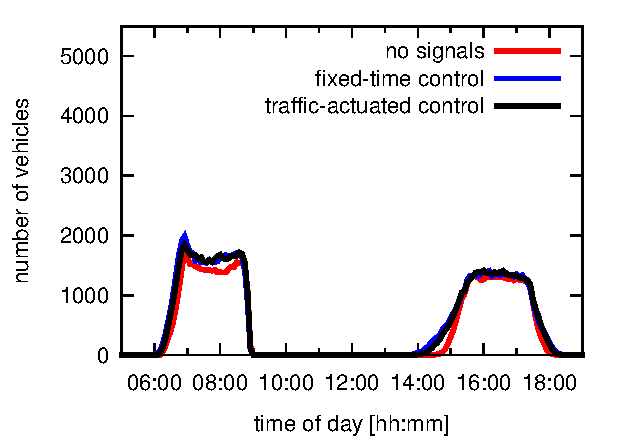
\includegraphics[width=0.48\linewidth]{extending/figures/signalslanes/leg_histogram_1292_1293_1291_it_1000.pdf}}
  {\label{fig:commuter_traffic}}%
  \createsubfigure%
	{Average travel time for unexpected event traffic, iteration 1000}
	{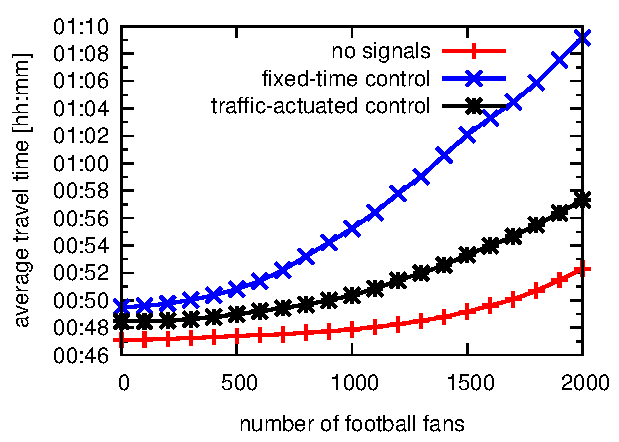
\includegraphics[width=0.48\linewidth]{extending/figures/signalslanes/average_travel_time_1220_1222.pdf}}
	{\label{fig:unexpected_event}}
}%
{\citet{Grether2014PhD}}

Simulation results for iteration 1000 of the Cottbus commuter scenario are depicted in
Fig.~\ref{fig:commuter_traffic}. 
The number of vehicles simultaneousely on the road is plotted over the time-of-day. 
%Due to the nature of a commuter scenario characterized by a steady
%demand over a certain time horizon 
The results are quite similar for all signal control strategies. 
The differences are small because of the lack of heavy congestion in the Cottbus scenario. 

A change of signal control has more effect if some unexpected traffic occurs in the network. 
It is assumed that the local soccer club ``FC Energie Cottbus'' has a derby that takes place on a normal weekday, thus interfering with the regular commuter traffic. 
In the last iteration of the run sequences, in addition to the commuters $0$ to $2000$ vehicles drive to the soccer stadium of Cottbus during the evening peak. 
It is assumed that 25 \% of these fans come from Cottbus,
while the other 75 \% come from the ``Spree-Nei{\ss}e'' area around Cottbus, and that all fans start their trips between 17:00 and 18:00. 

Fig.~\ref{fig:unexpected_event} plots the number of soccer fans on
the x-axis, and the average travel time of all travelers on the
y-axis. Without any additional vehicles,
the traffic-actuated signal control leads to a gain of
approx.~$1 \, min$ per traveler.
The more additional traffic is approaching the stadium, the more the traffic-actuated control saves travel time. In the case where 2000 additional vehicles are on the road, travel time savings reach ca.~$15\, min$~per traveler. 

Summarizing: Slightly jammed commuter scenarios, where a change in traffic signal control leads to heavily decreased overall travel time, have not been simulated with MATSim, yet. 
Looking at different objectives with more fine grained analysis tools can reveal network wide effects~\citep[e.g.~see the analysis using macroscopic fundamental diagrams, pp.114]{Grether2014PhD}, but this is work in progress.  
More heavily jammed scenarios can increase the overall traffic impact of a change in traffic signal control. Nevertheless the case study shows significant effects of traffic-responsive signal control, if something unexpected happens and travelers do not react.  

\subsection{Overview -- MATSim \& Traffic Signals}

The presented case study highlights some already researched aspects of MATSim simulations with traffic signals. 
MATSim is not the tool of choice for all questions concerning traffic signal control. 
The codebase, however, can also help to simulate other use cases, e.g.~evacuation or air transport scenarios. 
MATSim's open source nature provides hooks and interfaces for extension. 
But you should consider the amount of work required to get things done in respect to the current state of development and your project planning. 
The remaining chapter provides deeper insight.  
%If you need highly detailed traffic flow models or a high detail network representation, you should consider other tools. 
Sec.~\ref{sec:signals_traffic_signal_control} provides some traffic signal control backgrounds, vocabulary, and options for modeling with MATSim. More details can be found in the traffic signals user guide.  
Sec.~\ref{sec:signals_network_traffic_flow} goes into details of network and traffic flow modeling. 
If your requirements are met, Sec.~\ref{sec:signals_iterations_learning} considers iterations and learning. 
When it comes to agent based learning, MATSim is very fast -- the presented case study requires on average~$17$ seconds computation time per iteration -- for scoring, replanning, and output. One complete run sequence ($1000$ iterations, single core mobility simulation, multi core replanning) was simulated in $9 \, h$ and $12 \, min$. 
The speed of simulation leaves room for exploration of network wide behavioral reactions on changes of traffic signal control. 
Furthermore, the resource efficient simulation enables the joint simulation of several policies. 
Before you present your results to public, you should consider certain aspects concerning the  evaluation and interpretation of simulation results. 
Hints are provided in conjunction with a conclusion in Sec.~\ref{sec:signals_evaluation_conclusion}. 
%In Sec.~\ref{sec:signals_config} the most important configuration parameters are provided. 
%Thus, it is well worth to consider a extension for the simulation of traffic-responsive signal control. Further, the impacts of recently developed optimization models for fixed-time control can be tested~\citep{KoehlerStrehler2010SignalDemandOptimization}. 


\section{Traffic Signal Control}
\label{sec:signals_traffic_signal_control}

On a coarse level, control strategies for traffic signals can be classified in fixed-time and traffic-responsive strategies. 

Fixed-time traffic signal control periodically assigns green times for each approach of a junction. 
Cycle time and green split are not modified within short periods of time. 
To establish green waves between adjacent junctions the start of green light for the approaches within the cycle can be adjusted in respect to a global timer. 
These shifts are referred as coordination offsets. 
For optimization of fixed-time signals different regimes of equilibrium traffic flow are determined for several periods of time, e.g., weekday morning, midday, evening and night plus a separate estimate for weekends.   
Optimization may target all parameters of a signalized junction -- green split, cycle, offsets, and phase composition. 
%These traffic flows serve as input for optimization~\citep[e.g.~][]{Webster1961SignalSettings,Allsop1972SignalizedJunctionCapacity,Allsop1991SignalsStageBased,Robertson1969Transyt}.  
But, there is no possibility to react on current changes of equilibrium traffic flows. 

Traffic-responsive control reacts on current traffic patterns adjusting traffic signal control parameters on the fly. 
In principle all available information on prevailing traffic patterns can be used. 
The diversity of traffic-responsive control algorithms is wide, for a review the reader is referred to~\citet[][]{Grether2014PhD}. 

MATSim's traffic signal module is designed to simulate all different kinds of traffic signal control strategies. 
The module provides a default implementation for fixed-time control. 
Traffic-responsive strategies require custom implementation of the control algorithm but can make use of the existing data formats. 
Data is divided into five different types of input:
\begin{description}
	\item[Signals:] The location of the traffic signal hardware on the network is typically independent from the control strategy. Signals can be located at the end of a link or a lane, see the next section for further discussion of lanes. Signals are attached to a system that reflects e.g.~all signals of a junction or even larger units. Each signal system is controlled by exactly one control algorithm at a time.  
	\item[Signal Groups:] Traffic signals have to be attached to a group. A group of signals shows the same color at the same time. Each time a signal group changes its state a MATSim event is triggered. 
		There is no explicit representation of phases. If required this can be realized on top of the signal groups.  
	\item[Control:] A signal control comprises information for fixed-time control and can be used to specify custom control algorithms per system. 
	\item[Amber:] This input specifies the time of amber at the beginning and end of green time. At time of writing this information is only used for visualization purposes. 
		Driving is not permitted if a traffic signal shows amber light. 
	\item[Intergreens:] An intergreen time specifies the minimal time period between the ending of the one and the beginning of another signal group's green time.  
		This information is fairly important as MATSim's traffic flow model does not contain any collision detection. 
		When available, a validation module reads the event stream and triggers a warning or an error if security constraints are violated. 
		Further, customized control strategies can access this information to ensure the validity of control in respect to security aspects.    
\end{description}

For detailed information on the structure of those files and how to link them in the MATSim configuration file, we refer to the user guide in the contribution ``signals" which we update incrementally.

The next section considers network representation and location of traffic signals in more detail. 

%\mnote{Traffic-Actuated Control}
%With upcoming availability of sensors and computer technology these optimizations provided the basis for traffic-actuated signal control strategies. 
%Some actuated approaches use logical operators and functions to adjust signal timings~\citep{Friedrich2002VerkehrsadaptiveLSASteuerung}. More advanced methods as, e.g., SCOOT~\citep{HuntEtc1981SCOOT,RobertsonBretherton1991ScootMethod,BrethertonBodgerBaber2004ScootFuture}, MOTION~\citep{BielefeldtBusch1994MOTION,BuschKruse2001MotionSITRAFFIC,BrilonEtAl2009MotionMuenster}, or BALANCE~\citep{GEVAS2011Balance,BraunEtAl2009TravolutionLSA2CarCommunication} use macro- and mesoscopic traffic models to predict effects of adjustments of signal timings for a certain time horizon.  
%%
%
%%\mnote{Adaptive Control}
%Recent approaches for traffic signal control no longer need a fixed-time control that is adjusted. 
%Instead, the signal program is build completely on-the-fly based on sensor information.  
%%
%These methods originate from different areas of science. 
%One finds rather conceptual studies and methods that can and are used in practice. 
%%TUC
%An example for the latter is TUC (traffic-responsive urban control)~\citep{DiakakiPapageorgiouAboudolas2002MultivariableRegulatorTUC,DiakakiEtAl2003ExtensionsTUC,KrausEtAl2010CostEffectiveSignalsTUC,AboudolasEtAl2010RollingHorizonTUC,KouvelasEtAl2011HybridStrategyTUC} a control theoretic strategy that uses a linear-quadratic regulator approach to control green splits based on a store-and-forward model of urban traffic. 
%Due its polynomial complexity TUC can be used in real time monitoring the whole transport network. 
%Optional extensions to TUC provide cycle time adjustments, offset optimization, and public transit priority.   
%Also practice ready is the approach proposed by~\citet{Laemmer2007PhD,LaemmerHelbing2008SelfControlTrafficLights,LaemmerHelbing2010SelfStabilizingSignalControlRealNet}. 
%In undersaturated traffic conditions a priority based optimization of scheduling minimizes local waiting times. 
%A second module stabilizes the optimization when traffic density increases. 
%Green waves are established locally by a prediction model for future arrivals. 
%%
%Rather conceptual is the approach proposed by~\citet{CoolsEtAl2007SelfOrgSignalsSimulation,GershensonRosenblueth2009SelfOrgSignalsWithCA} that looks at traffic as a self-organizing system~\citep{ElmenreichEtAl2009SelfOrganizingSystemsSurvey}. 
%Traffic signals can be controlled by a set of simple rules, coordination evolves from the interaction between cars and signals. 
%Sensor information, however, can be erroneous as some detectors may not work at all or provide incorrect data. 
%If sensor data is erroneous, quality of an adaptive signal control may drop. 
%This problem is addressed by~\citet{OertelWagner2011DelayTimeActuatedSignals}. 
%Advanced traffic detection technologies as, e.g., GPS data or video processing, measure the delay imposed to individual vehicles approaching a signal. 
%When the delay is below a certain threshold a queue clearing policy terminates a green phase.  
%Noteworthy, in simulation studies, the signal control outperforms other approaches when only a part of the individual vehicle delays can be detected. 
%
%%\mnote{Agents}
%Intelligent agents~\citep{RusselNorvig2010ArtificialIntelligence} can be used to control traffic signals of one or several junctions~\citep{Bazzan2005signalAgents}. 
%Reinforcement learning techniques enable the agents to control traffic flows~\citep{Bazzan2005signalAgents,BazzanOliveiraSilva2010LearningTrafficSignals,Bazzan2009ReinforcementLearningPrint}.  
%Besides agent-based approaches, signalized junctions can be controlled by other techniques as autonomic and organic computing~\citep{Prothmann2010OrganicSignalControl}. 


\section{Network Representation \& Traffic Flow}
\label{sec:signals_network_traffic_flow}

\createfigure%
{Caption in List of Figures}%
{Transition from a real road segment to a graph layout with a single queue.}
{\label{fig:combined_model}}
{%
  \createsubfigure%
	{Typical real road layout}
	{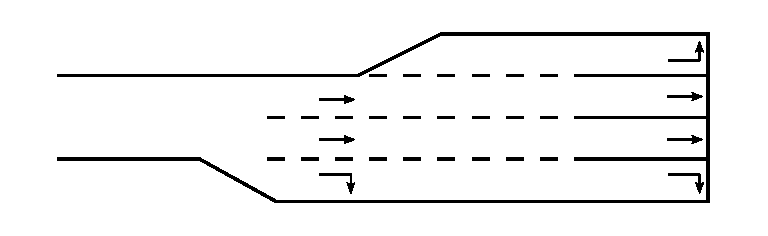
\includegraphics[width=0.475\linewidth]{extending/figures/signalslanes/real_road_layout.pdf}}
	{\label{fig:real_road_layout}}
  \createsubfigure%
	{Single queue, spill-back is not captured correctly}%
	{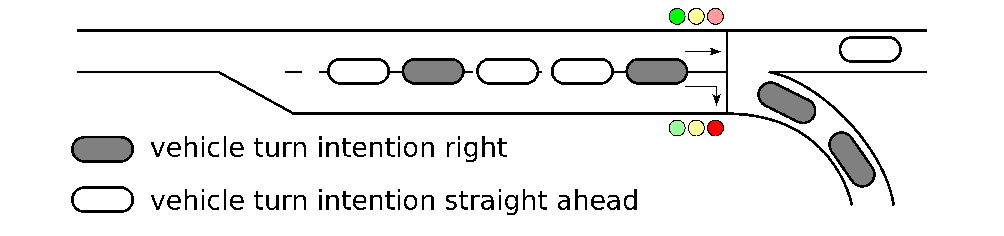
\includegraphics[width=0.48\textwidth]{extending/figures/signalslanes/single_queue_model_inkscape.pdf}}%
	{\label{fig:lanes_representation_single_queue}}%
}%
{\citet{Grether2014PhD}}

This section discusses the representation of transport networks with microscopically modeled traffic signals. 
In MATSim, the representation of the transport network is a static, directed graph consisting of nodes and links. 
Links depict road segments while nodes can be interpreted as decision points in space that have a coordinate as attribute, but no spatial dimension. 
%The location of nodes in space is not supposed to vary over time. 
%Nodes possess a geospatial interpretation and can be located in space. 
%But, in contrast to links, nodes have no spatial dimension.  
%The course of the road segments, however, is not specified and is inaccurate. 


Fig.~\ref{fig:real_road_layout} illustrates a typical layout of a real-world road segment with several turn pockets at its end. 
If the whole road segment is modeled as a single link with MATSim's queue model the first vehicle stopping at a red traffic signal at the end of this link will block all other vehicles approaching upstream, see Fig.~\ref{fig:lanes_representation_single_queue}. 
In respect to the road layout shown in Fig.~\ref{fig:real_road_layout} this is not realistic. 
Fig.~\ref{fig:model_link_layout} sketches the layout for a more realistic modeling. 
Vehicles with distinct turn intentions do not block each other until the available space for queueing on the turn pocket is used completely, see Fig.\ref{fig:lanes_representation_multiple_queue}. 

\createfigure%
{Caption in List of Figures}%
{Transition from a real road segment to a graph layout with multiple queues.}
{\label{fig:lanes_representation}}%
{%
  \createsubfigure%
	{Part of the graph required to model the road layout}
	{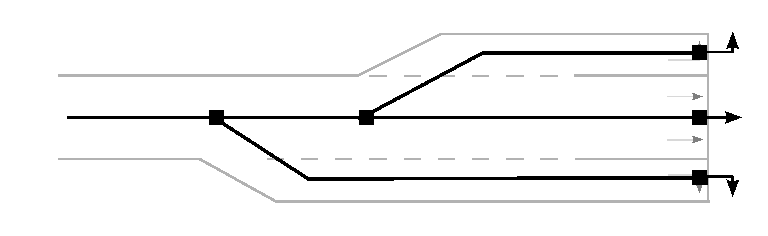
\includegraphics[width=0.475\textwidth]{extending/figures/signalslanes/link_lanes_layout}}
	{\label{fig:model_link_layout}}
  \createsubfigure%
	{Multiple queues, spill-back is captured correctly}%
	{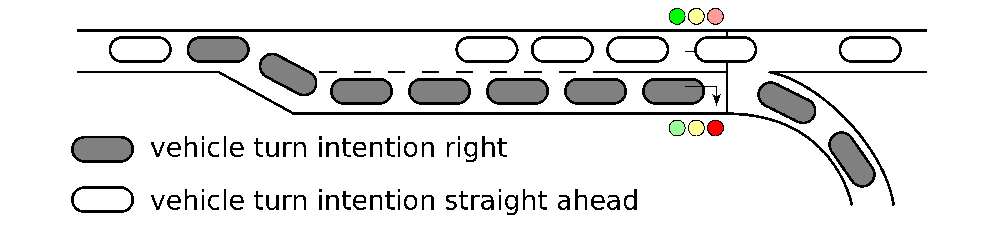
\includegraphics[width=0.48\textwidth]{extending/figures/signalslanes/multiple_queue_model_inkscape.pdf}}%
	{\label{fig:lanes_representation_multiple_queue}}%
}%
{\citet{Grether2014PhD}}

In principle you can model each turn pocket as link and put traffic signals at its end. 
But, considering overall project constraints, this has implications for network modeling and routing. 

In MATSim, all domain relevant attributes that differ from geospatial location, e.g.~traffic count data, transit stops, transit lines, or speed limits, are attached to links. 
If one of this attributes changes you have to model several links. 
Frequently, geospatial location of such attributes is not sufficient for an fully automatic matching between attributes and links. 
Some attributes and links require manual postprocessing. 
If you want to simulate traffic signals and turn pockets with an already existing scenario, spend some thoughts on your matching process before you change the network.  

MATSim specifies routes as sequences of links. 
Routes are generated by a shortest path algorithm that needs a cost function for links. 
In standard MATSim travel time on links is part of a link's cost.
While modeling turn pockets as links, the shortest path algorithm is responsible to select the appropriate turn pocket on a route.
If your modeling includes turn restrictions, make sure that they are captured by the shortest path algorithm. 
Besides, the required number of iterations increases if many turn pockets lead to the same downstream link. 
So, it is important that you understand the interaction of route generation and network modeling if you model turn pockets as links. 

If the network modeling or routing issues conflicts with other goals of your project, there is an alternative available. 
MATSim allows the modeling of a subgraph on top of each link that reflects the structure shown in Fig.~\ref{fig:model_link_layout}. 
The links of the subgraph are then called \emph{lanes}. 
At the beginning of a link only one lane is necessary. 
But at the end of a link different lanes may exist to model the available turn pockets. 
So, for a vehicle it is necessary to be in the correct turning lane for the next downstream link of it's route.
If there is more than one lane leading to the next downstream link the vehicle is placed on the lane that currently contains the smallest number of other vehicles. % if there are several lanes leading to the same downstream link. 
Specific turning moves can be forbidden. 
If lanes are used, the shortest path algorithm is set up on the line graph of the original network graph.  
Thereby, the turn restrictions are considered when the line graph is created. 
%The dynamic link travel times for the line graph reflect the link travel time on the original network plus the travel time for the specific turning move. 
The shortest path calculation captures the effects of lanes without further modification. 
%In addition, turn restrictions cannot be captured by standard shortest path algorithms. 

Besides the mentioned differences lanes behave similar or equal to links.  
Traffic signals can be placed at the end of links and lanes. 
Traffic on each lane is simulated the same way as for links. 
Traffic flow increases linear in the green time of a signal. 
Vehicles entering or leaving lanes trigger events that possess the same structure and information as link enter and leave events.

At the end it is up to you to use lanes or not. 
Most MATSim scenarios with signals are set up using lanes, the codebase is considered well debugged. 
Without lanes the code for traffic signals is also tested, but you should double check the routing for artefacts. 

\section{Iterations \& Learning}
\label{sec:signals_iterations_learning}

This section discusses the interaction between traffic signals and travelers within the MATSim iteration cycle. 

\citet{Meneguzzer1997ModelReviewTrafficAssignmentSignalControl} defines the {\bf combined traffic assignment and control problem} (CTAC) as finding a tuple $(f^{*}, g^{*})$ of traffic flows $f$ and signal settings $g$ under policy $P$ that fulfills  
\[
f^{*} = f^{e}[g^{P}(f^{*})] \mbox{  or  equivalently } g^{*} = g^{P}[f^{e}(g^{*})]
\]
where $f^{e}$ is a function mapping signal settings to equilibrium traffic flows and $g^{P}$ a function mapping traffic flows to signal settings under policy $P$.  
Nicely, the formulation shows the mutual interaction of traffic patterns and signal settings. 
%A similar problem formulation is given by~\citet{CascettaGalloMontella2006SignalsWithStochAssignment}, studying the difference between global and local signal optimization. 
The time horizon, on that these interactions take place, is not captured by the formulations. 

The interpretation of traffic signals within the MATSim iteration cycle depends strongly on the type of signal control and your interpretation of the learning mechanism. 
For a fixed-time control the fixed-point interpretation can be valid, at least if you do not expect something unexpected. 
For traffic-actuated signal control strategies no standard interpretation can be provided. 
Readers willing to dig deeper are referred to~\citet[pp.~75][]{Grether2014PhD}.  
Here we conclude with the advice to document clearly what and how you have simulated and provide an interpretation that makes sense from your point of view.    

\section{Conclusion} %{Traffic Signals in MATSim}
\label{sec:signals_evaluation_conclusion}

Before we conclude, a few thoughts on evaluation of traffic signal control. 
MATSim can simulate traffic signal control microscopically. 
But, certain effects of traffic signals are not represented by MATSim without further customization and implementation, e.g.~microscopic de- and acceleration as reaction on traffic control. 
So check your evaluation and interpretation against your simulation setup. 

After reading this chapter you got an overview of traffic signals in MATSim. 
You know what to consider before you make your first steps in a larger scenario. 
As technical documentation outdates quickly the chapter tries to avoid technical details as there is also an incrementally improving user guide\footnote{Find the user guide  in the contribution ``signals'' where in future days the package \lstinline|signalsystems| is moved}.  
We think that MATSim is a great tool if it comes to microscopic simulated traffic-responsive signal control that shall be analyzed network wide assuming heterogeneous user reactions. 


%\section{Automatically Generated Module Information}
%\label{sec:signals_config}
%Module in the config: 
%\begin{itemize}
%	\item \lstinline|signalsystems|
%\end{itemize}
%
%Package:
%\begin{itemize}
%	\item \lstinline|org.matsim.signalsystems|
%\end{itemize}
%
%http://matsim.org/node/732
%
%Literature: \citet[][]{GretherEtAl_ABMTRANS_2012, Grether_PhDThesis_2014, Neumann_MastersThesis_2008}
%Auch Miss Ou-Paper ansehen: Optimierung von Lichtsignalen
%
%\citet[][p.?]{BalmerEtAl_ResRep_bdktzrh_2009}
%
%
%Information about signal light timing are available for the city of Zurich  \citep{STAPOZH-DAV_unpub_gtZH_2008} (\ref{ptl:zhCity}). Modeling of traffic lights was implemented for the project \emph{Westumfahrung} trough reducing the available link capacity. However, the used \emph{mobsim} (DEQSim) is deprecated (see Section \ref{sec:deqsim}).
%
%Research and implementation efforts are undertaken to include individual traffic lights in other \emph{mobsims} (see e.g., (\ref{tl:docu}) and \citet[][]{Neumann_MastersThesis_2008}).
%
%% -------------------------------------------
%
%Lanes:
%
%The lanes package has been implemented in conjunction with signal systems. Lanes are enabled in the \lstinline|scenario| configuration file section. The lanes package (\lstinline| org.matsim.lanes|) provides readers, where the class \lstinline|ModelLane| serves as the interface between the lane functionality and the mobility simulation. The lane definitions file needs to be specified in the \lstinline|network| configuration file section.

% ##################################################################################################################
